\section{闭区间上可微函数的性质}
\label{sec:ru-interval-differentiable}

导数记录一点处的变化率。本节把它与区间上的极值、净变化、增减方向、弯曲方向以及变化幅度联系起来。
主要对象是在闭区间上连续、在区间内部可微的函数；局部极值与驻点先在内点讨论，各结论分别写明是否需要端点连续、单侧导数或导数的界。

\subsection{局部极值与驻点}
\label{sec:ru-local-extrema}

导数只反映一点附近的变化，与它对应的是只比较邻近函数值的极值。设$c$属于$f$的定义域，若存在$r>0$，使定义域中满足$|x-c|<r$的$x$都有$f(x)\geq f(c)$，
则称$c$为$f$的局部极小点；若其中$x\neq c$的点都满足$f(x)>f(c)$，称为严格局部极小点。不等号反向，得到局部极大点。
局部极值只与附近比较，整个定义域上的最值则与全部输入比较；最小点一定是局部极小点，反之不然。
\begin{theorem}[Fermat定理]
\label{thm:analysis-fermat}
设$c$是区间$I$的内点，$f:I\to\mathbb R$在$c$处可导。若$c$为$f$的局部极小点或局部极大点，则
\begin{equation}
 f'(c)=0.
 \label{eq:analysis-scalar-first-order-necessary}
\end{equation}
\end{theorem}
\begin{proof}
设$c$为局部极小点。充分小的$h\neq0$满足$f(c+h)-f(c)\geq0$，所以$h>0$时差商非负，$h<0$时差商非正。两侧差商趋于同一个导数，于是$f'(c)\geq0$且$f'(c)\leq0$。局部极大点对$-f$论证。
\end{proof}
导数为零的点称为\term{驻点}（stationary point）。Fermat定理说明，内点处可导的局部极值点必为驻点。证明用到了从两侧取差商，所以结论只适用于内点。

在闭区间上找最值时，极值定理保证最值存在，Fermat定理则缩小了候选范围：最值点只可能是端点、内部驻点，或者内部不可导的点。
例如$f(x)=x^3-3x$在$[-2,3]$上，$f'(x)=3(x-1)(x+1)$，驻点为$\pm1$。比较$f(-2)=-2$、$f(-1)=2$、$f(1)=-2$、$f(3)=18$，最大值$18$在端点$3$取得，最小值$-2$在$-2$与$1$两处取得。
导数为零只是内点极值的必要条件。$x^3$在$0$处导数为零，但$x<0$时$x^3<0$、$x>0$时$x^3>0$，$0$不是极值点。
不可导的点也要单独检查：$|x|$在$0$处取最小值，那里没有导数；端点$0$是$x$在$[0,1]$上的最小点，右导数却是$1$。

\subsection{中值定理}
\label{sec:ru-mean-value-theorems}

若函数在区间两端取同一值，整段的净变化为零；在连续、可导的条件下，区间内部必有一点的瞬时变化率也为零。
\begin{theorem}[Rolle定理]
\label{thm:analysis-rolle}
设$a<b$，$f$在$[a,b]$上连续、在$(a,b)$内可导，且$f(a)=f(b)$，则存在$c\in(a,b)$使$f'(c)=0$。
\end{theorem}
\begin{proof}
若$f$为常数，任取$c$即可。否则$f$在某个内点的值不同于$f(a)$。由极值定理，$f$在$[a,b]$上达到最大值和最小值，其中至少有一个与端点值不同，因而在某个内点$c$取得。
$c$是局部极值点，$f$在那里可导，由Fermat定理$f'(c)=0$。
\end{proof}
两端取值不同时，先减去连接两端点的直线，使剩余部分在两端相等，再用Rolle定理。
\begin{theorem}[Lagrange中值定理]
\label{thm:analysis-lagrange-mean-value}
设$a<b$，$f$在$[a,b]$上连续、在$(a,b)$内可导，则存在$c\in(a,b)$使
\begin{equation}
 f(b)-f(a)=f'(c)(b-a).
 \label{eq:analysis-mean-value-theorem}
\end{equation}
\end{theorem}
\begin{proof}
令$H(x)=f(x)-f(a)-\frac{f(b)-f(a)}{b-a}(x-a)$，则$H$满足Rolle定理的条件，且$H(a)=H(b)=0$。由$H'(c)=0$整理即得。
\end{proof}
这就是\term{中值定理}（mean value theorem）的含义：区间上的平均变化率等于某个内点处的瞬时变化率。定理只要求内点可导，不要求导函数连续，也不要求端点的单侧导数存在。
图~\ref{fig:analysis-process-mean-value-parallel}以$f(x)=x^2$、区间$[0,1]$为例：端点割线的斜率为$1$，$c=1/2$处的切线与之平行。

\begin{figure}[!htbp]
 \centering
 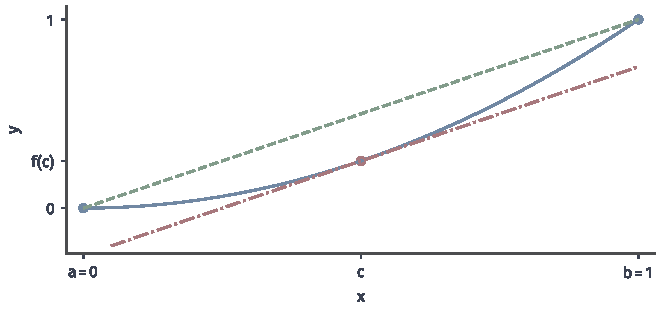
\includegraphics[width=112.0mm]{figures/01-mathematical-preliminaries-upper/00-shared/matplotlib/chapter3-concept-processes/mean-value-parallel.pdf}
 \caption{$f(x)=x^2$在$[0,1]$上，绿虚线为端点割线，红点划线为$c=1/2$处的切线。两线平行，因为$f'(c)=1=[f(1)-f(0)]/(1-0)$。两线高度不同：相等的是斜率，两条直线并不重合。}
 \label{fig:analysis-process-mean-value-parallel}
\end{figure}

比较两个函数在同一区间上的变化时，可以把两者的端点增量放进同一个辅助函数。结论先写成交叉相乘的形式，不需要假设任何分母非零。
\begin{theorem}[Cauchy中值定理]
\label{thm:analysis-cauchy-mean-value}
设$a<b$，$f,g$都在$[a,b]$上连续、在$(a,b)$内可导，则存在$c\in(a,b)$使
\[
 \bigl(f(b)-f(a)\bigr)g'(c)=\bigl(g(b)-g(a)\bigr)f'(c).
\]
若还有$g'(x)\neq0$对每个$x\in(a,b)$成立，则$g(b)\neq g(a)$，并且
\[
 \frac{f(b)-f(a)}{g(b)-g(a)}=\frac{f'(c)}{g'(c)}.
\]
\end{theorem}
\begin{proof}
令$H(x)=(f(b)-f(a))(g(x)-g(a))-(g(b)-g(a))(f(x)-f(a))$，则$H(a)=H(b)=0$，由Rolle定理得$H'(c)=0$，展开即为交叉相乘形式。
若$g'$在内部处处非零，$g(b)=g(a)$会使Rolle定理给出某个内点处$g'=0$，所以$g(b)\neq g(a)$；两边同除以非零的$(g(b)-g(a))g'(c)$即得比值形式。
\end{proof}
取$g(x)=x$即回到Lagrange中值定理。写成比值时要先检查分母：比值形式依赖$g'$在内部处处非零，第~\ref{sec:ru-lhopital}节的L'Hôpital法则正是用这一形式证明的。

\subsection{单调性与凹凸性}
\label{sec:ru-monotonicity-convexity}
\label{sec:analysis-monotonicity}

中值定理把任意两点之间的增量写成某个内点处的导数乘以输入增量，所以导数的符号可以控制整段的增减。
\begin{theorem}[导数符号与单调性]
\label{thm:analysis-derivative-monotonicity}
设$f$在区间$[a,b]$上连续、在$(a,b)$内可导。若在$(a,b)$内$f'\geq0$，则$f$在$[a,b]$上单调不减；若$f'>0$，则严格递增。$f'\leq0$与$f'<0$相应地给出单调不增与严格递减；若$f'\equiv0$，则$f$为常数。
\end{theorem}
\begin{proof}
任取$a\leq x<y\leq b$，在$[x,y]$上用Lagrange中值定理，$f(y)-f(x)=f'(\xi)(y-x)$，右侧的符号由$f'(\xi)$决定。
\end{proof}
关键是两点之间的整段都属于定义域。在$(0,1)\cup(2,3)$上左段取$0$、右段取$1$的函数导数处处为零，却不是常数，中值定理不能跨过定义域的缺口。
导数处处为正是严格递增的充分条件而非必要条件：$x^3$在$\mathbb R$上严格递增，但在$0$处导数为零。

同样的论证可以判断驻点是否为极值：若$f'$在$c$左侧为负、右侧为正，则$f$在$c$左侧严格递减、右侧严格递增，$c$是严格局部极小点；左正右负则为严格局部极大点。
例如$x^3-3x$的导数$3(x-1)(x+1)$在$1$的左侧为负、右侧为正，$1$是严格局部极小点；在$-1$两侧由正变负，$-1$是严格局部极大点。
若导数在驻点两侧同号，如$x^3$在$0$两侧都有$3x^2>0$，函数沿同一方向变化，驻点就不是极值点。

函数自身的单调性由$f'$的符号决定；$f'$本身的单调性则描述图像的弯曲方向。在区间上任取两点，连接图像上对应两点的线段称为弦。
\begin{definition}[凸函数]
\label{def:ru-convex-function}
设$f$定义在区间$I$上。若对任意$x,y\in I$与$\lambda\in[0,1]$，都有
\[
 f\bigl(\lambda x+(1-\lambda)y\bigr)\leq\lambda f(x)+(1-\lambda)f(y),
\]
即两点之间的图像不高于弦，就称$f$为\term{凸函数}（convex function）；$x\neq y$、$0<\lambda<1$时不等式总是严格成立，称为严格凸函数。若$-f$是凸函数，称$f$为凹函数。
\end{definition}
例如$x^2$是凸函数：$\lambda x^2+(1-\lambda)y^2-(\lambda x+(1-\lambda)y)^2=\lambda(1-\lambda)(x-y)^2\geq0$，并且$x\neq y$时严格大于零。

\begin{theorem}[可微凸函数的刻画]
\label{thm:ru-convexity-derivative}
设$f$在开区间$I$上可微，则下面三条等价：
(1) $f$是凸函数；(2) $f'$在$I$上单调不减；(3) 对任意$x,y\in I$，$f(y)\geq f(x)+f'(x)(y-x)$，即图像总在每条切线的上方。
\end{theorem}
\begin{proof}
(1)$\Rightarrow$(2)：设$x<z<y$，把$z$写成$\lambda x+(1-\lambda)y$，其中$\lambda=(y-z)/(y-x)$，凸性不等式整理后就是三条弦的斜率关系
\[
 \frac{f(z)-f(x)}{z-x}\leq\frac{f(y)-f(x)}{y-x}\leq\frac{f(y)-f(z)}{y-z}.
\]
令$z\to x^+$，左边趋于$f'(x)$；令$z\to y^-$，右边趋于$f'(y)$。所以$f'(x)\leq\frac{f(y)-f(x)}{y-x}\leq f'(y)$。

(2)$\Rightarrow$(3)：由中值定理，$f(y)-f(x)=f'(\xi)(y-x)$，$\xi$在$x,y$之间。$y>x$时$\xi>x$，$f'(\xi)\geq f'(x)$，所以$f(y)-f(x)\geq f'(x)(y-x)$；$y<x$时$f'(\xi)\leq f'(x)$而$y-x<0$，结论相同。

(3)$\Rightarrow$(1)：令$z=\lambda x+(1-\lambda)y$，在$z$处的切线不等式给出$f(x)\geq f(z)+f'(z)(x-z)$与$f(y)\geq f(z)+f'(z)(y-z)$。
两式分别乘以$\lambda$与$1-\lambda$再相加，右侧的一次项因$\lambda(x-z)+(1-\lambda)(y-z)=0$而消去，得到$\lambda f(x)+(1-\lambda)f(y)\geq f(z)$。
\end{proof}
图~\ref{fig:ru-convex-chord-tangent}画出了凸函数与它的一条弦和一条切线：弦在图像上方，切线在图像下方。
凸性要求的是$f'$单调不减，而不是$f$单调：$x^2$在$\mathbb R$上不单调，却是凸函数。

\begin{figure}[!htbp]
 \centering
 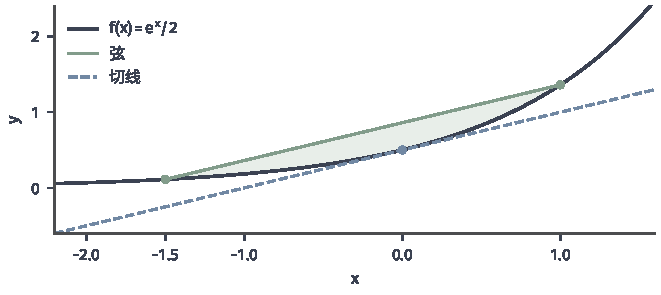
\includegraphics[width=112mm]{figures/01-mathematical-preliminaries-upper/02-real-numbers-and-univariate-functions/matplotlib/convex-chord-tangent/figure.pdf}
 \caption{凸函数$f(x)=e^{x}/2$的弦与切线。绿线连接$x=-1.5$与$x=1$处的两点，两点之间的图像在弦的下方；蓝线是$x=0$处的切线$y=\tfrac12+\tfrac12x$，整条图像在它的上方。图为解析示例。}
 \label{fig:ru-convex-chord-tangent}
\end{figure}

在二阶可微的条件下，凸性可以由二阶导数判断。若$f$在开区间$I$上二阶可导且$f''\geq0$，由定理~\ref{thm:analysis-derivative-monotonicity}，$f'$单调不减，所以$f$是凸函数；
若$f''>0$，则$f'$严格递增，把上面证明中的不等号改为严格，可知$f$严格凸。反方向只对非严格情形成立：凸函数满足$f''\geq0$，因为单调不减的$f'$的导数非负。
严格凸却不要求$f''$处处严格为正。$x^4$的导数$4x^3$在$\mathbb R$上严格递增，所以$x^4$严格凸，但$f''(0)=0$。“二阶导数处处为正”是严格凸的充分条件，不是必要条件。
二阶导数也能判断驻点：若$f'(c)=0$且$f''(c)>0$，则$f'(c+h)/h\to f''(c)>0$，充分小的$h$使$f'(c+h)$与$h$同号，由一阶判别，$c$是严格局部极小点；$f''(c)<0$时是严格局部极大点。
$f''(c)=0$时没有结论：$x^4$、$-x^4$与$x^3$在原点的一、二阶导数都为零，原点分别是极小点、极大点和非极值点。

最后，若导数有统一的界，中值定理把它转化为变化幅度的界。
\begin{theorem}[有界导数与Lipschitz条件]
\label{thm:analysis-bounded-derivative-lipschitz}
设$f$在$[a,b]$上连续、在$(a,b)$内可导，且$|f'(x)|\leq L$对所有$x\in(a,b)$成立，则对任意$x,y\in[a,b]$，$|f(y)-f(x)|\leq L|y-x|$。
\end{theorem}
\begin{proof}
$x\neq y$时，由中值定理$|f(y)-f(x)|=|f'(\xi)|\,|y-x|\leq L|y-x|$。
\end{proof}
例如$\sin$的导数绝对值不超过$1$，所以$|\sin x-\sin y|\leq|x-y|$对所有实数成立。闭区间上的$C^1$函数，导数连续因而有界，于是都是Lipschitz函数。
这说明局部导数信息在具备区间条件时可以给出整体控制。反过来，Lipschitz连续不保证可导：$|x|$在$[-1,1]$上的Lipschitz常数为$1$，在$0$处却不可导。
一元凸性的这些结论将在最优化部分推广到多元函数，并用于判断最优点（第~\ref{chap:optimization}章）。
